\documentclass{beamer}

\usepackage[frenchb]{babel}
\usepackage[T1]{fontenc}
\usepackage[utf8]{inputenc}
\usetheme{Warsaw}


\usepackage{amsmath}
\usepackage{amssymb}
\usepackage{amsthm}
\usepackage{stmaryrd}

\usepackage[all]{xy}

\setbeamercovered{transparent}

\begin{document}

\title{Monades, Comonades et Automates cellulaires}
\author{Jérémy S. Cochoy}
\institute{INRIA Paris-Saclay}
\date{Octobre 2015}


\begin{frame}
\titlepage
\end{frame}

\begin{frame}
\tableofcontents
\end{frame}

\begin{frame}

\begin{center}

\includegraphics[scale=0.3]{screen1.png}
\end{center}

\end{frame}

\section{Monades}

\subsection{Types}
\begin{frame}
\frametitle{Les types}
\begin{block}{Qu'est-ce qu'un type?}
C'est un \emph{ensemble} de valeurs.
\end{block}
\pause
\begin{exampleblock}{Examples :}
\begin{itemize}
\item $Int = \{-2 147 483 648, \dots, 2 147 483 647\}$
\item $Bool = \{True, False\}$
\item $Char = \{'a', 'b', 'c' , \dots\}$
\pause
\item $[Bool] = \{[], [True], [False], [True, False], [False, True], \dots\}$
\pause
\item $[a]$
\end{itemize}

\end{exampleblock}
\end{frame}

\begin{frame}
\frametitle{Les types}
\begin{block}{Construire son type :}
\begin{itemize}
\item Trival = Plus | Minus | Zero
\pause
\item Box a = InABox a
\pause
\item Maybe a = Just a | Nothing
\pause
\item Either a b = Left a | Right b
\end{itemize}
\end{block}

\pause

Just, Nothing, InABox etc portent le doux nom de \emph{constructeur de type}. C'est aussi le cas de \emph{[]}.
\end{frame}

\subsection{Fonctions}
\begin{frame}
\frametitle{Les fonctions}
\begin{block}{}
Ce sont les traitements que l'on peux implémenter.
\end{block}
\begin{center}

\includegraphics[scale=0.2]{fct.png}
\end{center}
\pause
\begin{block}{}
Une fonction ne lance pas de fusé.
\end{block}
\end{frame}


\begin{frame}
\frametitle{Les fonctions}
\begin{block}{Une fonction a aussi un type : \emph{a -> b}}
\begin{itemize}
\item floor   :: Float -> Int
\item (+2):: Int -> Int
\pause
\item id      :: a -> a
\item map :: (a -> b) -> [a] -> [b]
\end{itemize}
\end{block}

\end{frame}


\begin{frame}
\frametitle{Les fonctions}
\begin{block}{Ça se compose}
\begin{itemize}
\item f1 :: a -> b
\item f2 :: b -> c
\item f2 . f1 :: a -> c
\pause
\item . :: (a -> b) -> (b -> c) -> (a -> c)
\end{itemize}
\end{block}
\pause

Pour l’anecdote, la collection de tous les types forme une catégorie où les flèches sont les fonctions implémentables. On l’appelle la catégorie des types.

\end{frame}

\subsection{Foncteurs}

\begin{frame}
\frametitle{Donnée dans un contexte}

\begin{block}{}
Un foncteur place une valeur dans un contexte.
\end{block}

\begin{center}
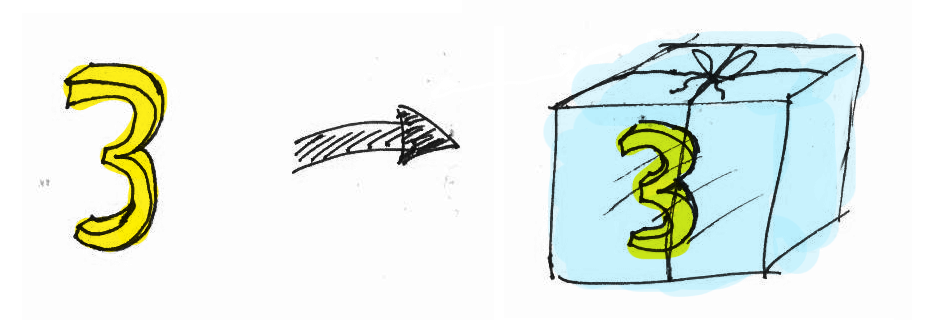
\includegraphics[scale=0.3]{just3.png}
\end{center}

\begin{exampleblock}{}
L'exemple de Maybe : \verb!Just 3!
\end{exampleblock}
\end{frame}

\begin{frame}
\frametitle{Donnée dans un contexte}

\begin{block}{}
Un contexte peux aussi ne pas contenir de valeur.
\end{block}

\begin{center}
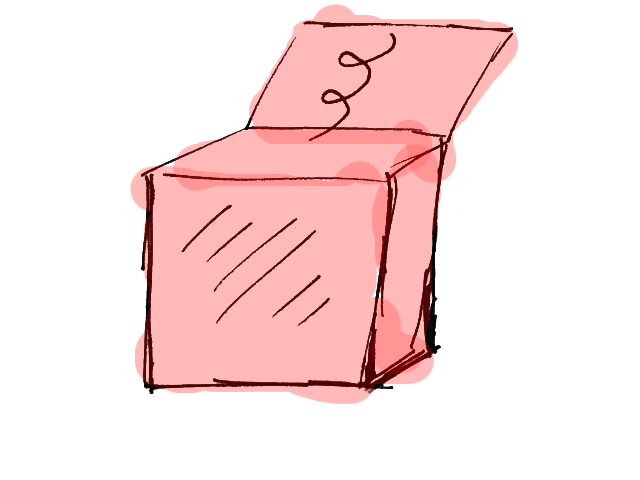
\includegraphics[scale=0.3]{nothing.png}
\end{center}
\begin{exampleblock}{}
L'exemple de Maybe : \verb!Nothing!
\end{exampleblock}
\end{frame}

\begin{frame}
\frametitle{Functorial mapping}
On ne peux plus appliquer la fonction telle quelle.
\begin{center}
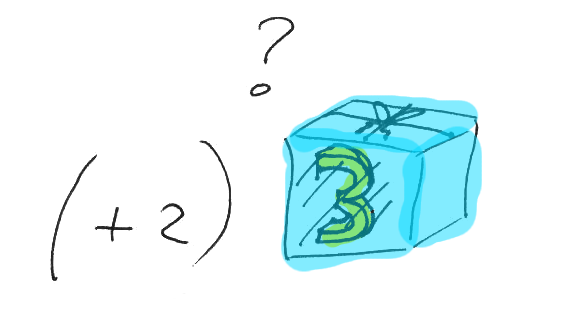
\includegraphics[scale=0.3]{wrong_type.png}
\end{center}
\end{frame}

\begin{frame}
\frametitle{Functorial mapping}
Mais le foncteur nous donne une nouvelle flèche.
\begin{center}
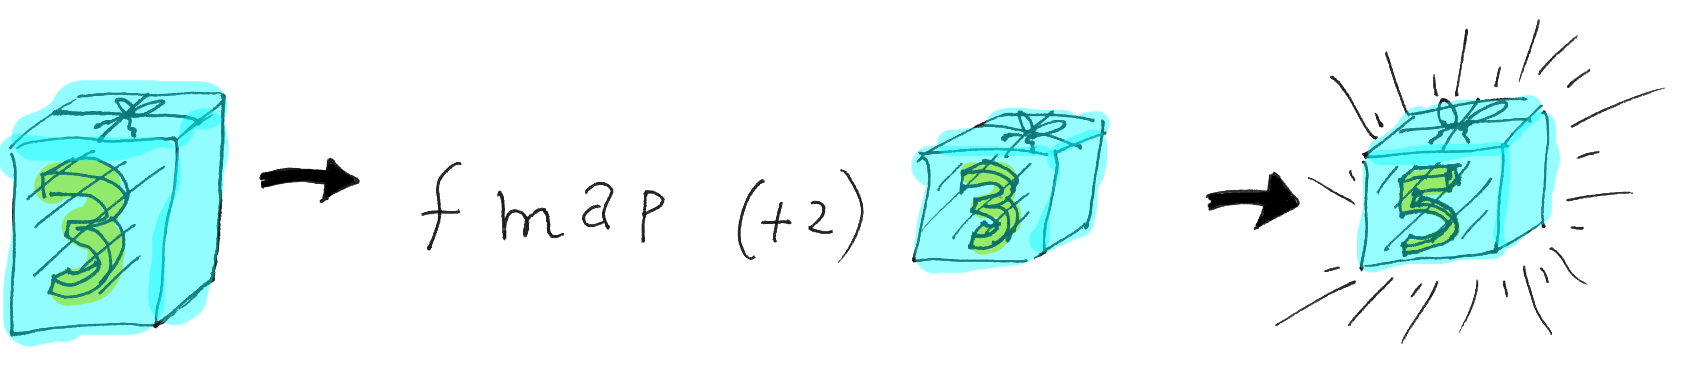
\includegraphics[scale=0.19]{f_fct.png}
\end{center}
\end{frame}


\begin{frame}
\frametitle{Les foncteurs}
\begin{block}{Un foncteur F agit sur les types ...}
\begin{itemize}
\item a => F a
\end{itemize}
\end{block}
\begin{exampleblock}{}
\begin{itemize}
\item a => Maybe a
\item a => [a]
\end{itemize}
\end{exampleblock}

\pause

\begin{block}{... et sur les fonctions}
\begin{itemize}
\item a -> b => F a -> F b
\end{itemize}
\end{block}

\begin{exampleblock}{}
\begin{itemize}
\item fmap (+2) :: F Int -> F Int
\item fmap id :: F a -> F a
\end{itemize}
\end{exampleblock}
\end{frame}


\begin{frame}
\frametitle{Dura lex sed lex}
\begin{alertblock}{Un foncteur doit respecter des lois}
\begin{itemize}
\item fmap id = id
\item fmap (p . q) = (fmap p) . (fmap q)

\end{itemize}
\end{alertblock}

\pause
Un foncteur est un endofoncteur de la catégorie des types.
\end{frame}



\begin{frame}
\frametitle{Un traitement qui peux échouer}

\begin{center}
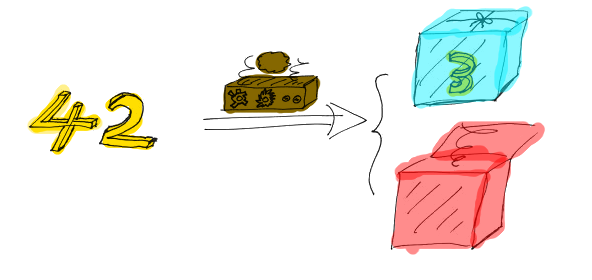
\includegraphics[scale=0.5]{failure.png}
\end{center}
\begin{exampleblock}{}
Une fonction de type \emph{Int -> Maybe Int}.
\end{exampleblock}
\end{frame}

\begin{frame}
\frametitle{Combiner des traitements avec échec}
\end{frame}

\begin{frame}
\frametitle{L'opérateur bind}
\end{frame}


\begin{frame}
\frametitle{L'opérateur join}
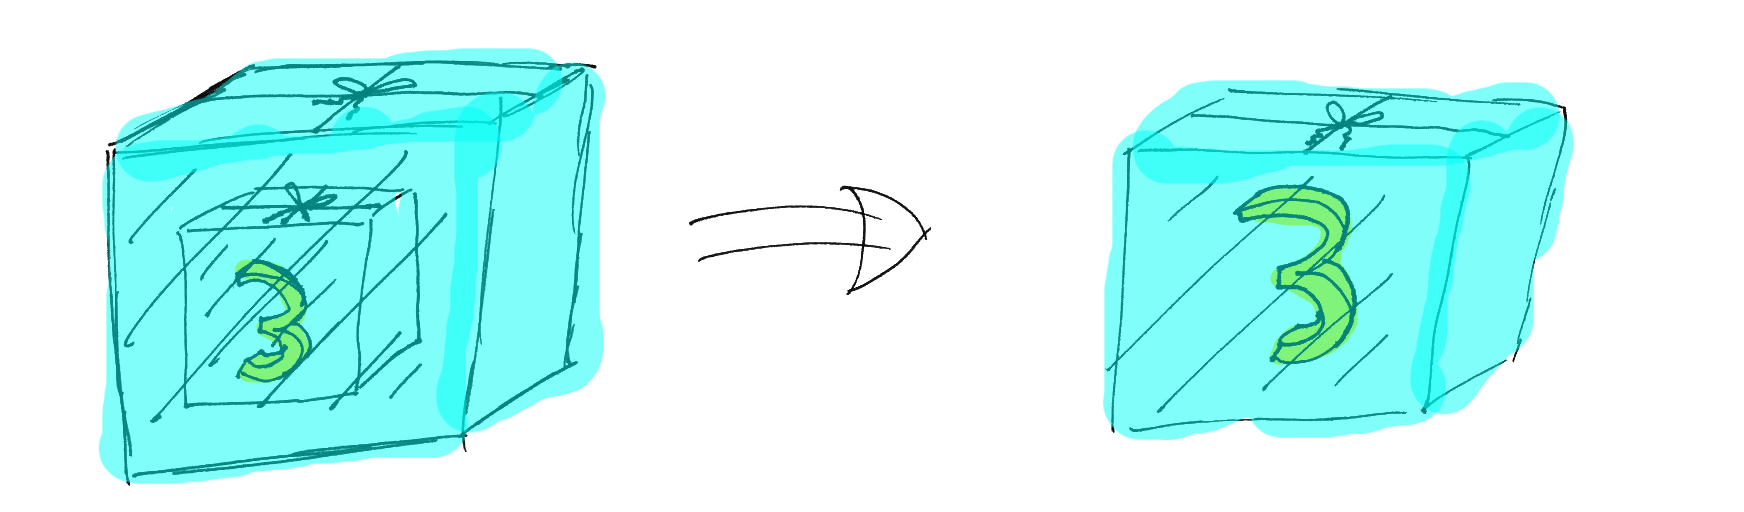
\includegraphics[scale=0.2]{join.png}
\end{frame}

\begin{frame}
\frametitle{L'opérateur join}
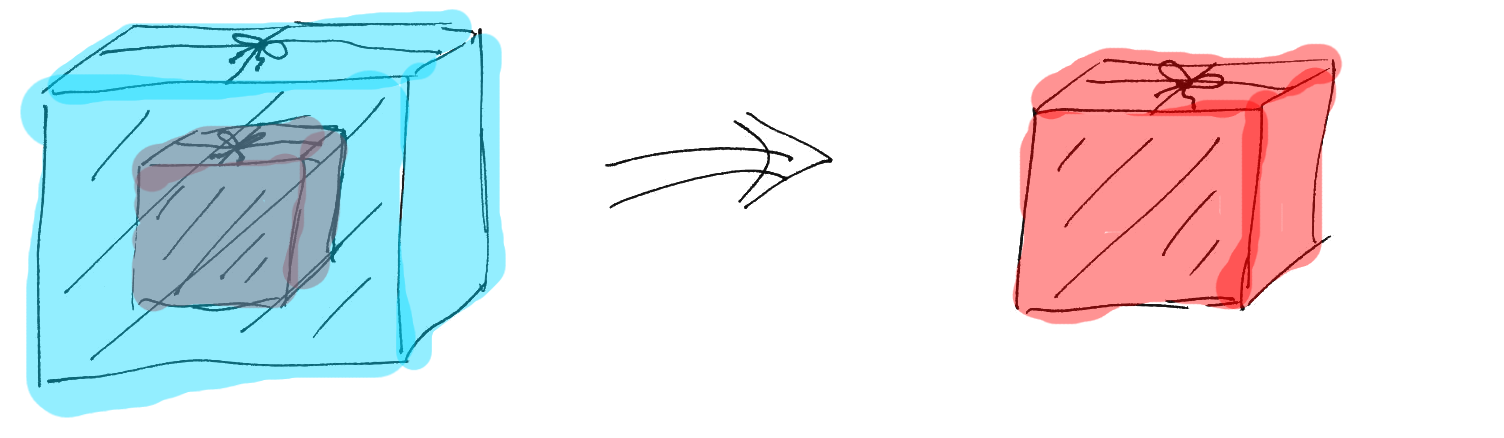
\includegraphics[scale=0.2]{join_nothing.png}
\end{frame}

\begin{frame}
\frametitle{Monade}
\end{frame}

\begin{frame}
\frametitle{Monades - Catégories}
Une monade $(T, \mu, \eta)$ est la donné d'un
endofoncteur $T : C \rightarrow C$ et de deux
transformations naturelles $\mu : T\circ T \rightarrow T$ et $\eta : 1_C \rightarrow T$ telles que :

\[
\xymatrix{
T(T(T(X))) \ar[r]^{T(\mu_X)} \ar[d]_{\mu_{T(X)}} & T(T(X)) \ar[d]^{\mu_X} \\
T(T(X)) \ar[r]_{\mu_X} & T(X) \\
}
\]
\[
\xymatrix{
T(X) \ar[r]^{\eta_{T(X)}} \ar[d]_{T(\eta_X)}  \ar@{=}[dr] & T(T(X)) \ar[d]^{\mu_X} \\
T(T(X)) \ar[r]_{\mu_X} & T(X) \\
}
\]
c'est à dire
$\mu \circ T\mu = \mu \circ \mu T$
et
$\mu \circ T \eta = \mu \circ \eta T = 1_T$.

\pause

Dans notre cas, $C$ est la catégorie des types ; les objet sont les ensembles de valeurs que peuvent prendre une fonction ($Int = {-32768 , \dots, 32767}$), et les flèches sont les fonctions ($f :: Int -> Int$).
\end{frame}

\section{Automates Cellulaires}
\begin{frame}
\end{frame}

\section{Comonades}
\begin{frame}
\end{frame}

\end{document}
